\documentclass[12pt,letterpaper]{article}


\newcommand{\studentname}{Ben Bassett}
\newcommand{\labpartner}{Katrina Sumarli}

\title{\textsc{Lab 01: Beads in a Jar}}
\newcommand{\shorttitle}{Beads in a Jar}

\newcommand{\course}{PHY310}
\newcommand{\labdate}{09-03-2024}

%------------------------------------------------------------------------------------------------------------

\usepackage[letterpaper,left=1in,right=1in,bottom=1in,top=1in]{geometry}
\usepackage{fancyhdr}
\usepackage{subfigure}
\usepackage{graphicx}
\usepackage{amsmath}
\usepackage{cleveref}
\usepackage{booktabs}
\usepackage[british]{babel}
\usepackage[square,comma,numbers,sort&compress]{natbib}
\usepackage{csvsimple}
\usepackage{graphicx}
\usepackage{pgfplotstable}
\usepackage{textcomp,gensymb}
\usepackage{array}
\usepackage{tabu}
\usepackage{multirow}
\usepackage{url}
\pgfplotsset{compat=1.9}% supress warning
\begin{document}

%------------------------------------------------------------------------------------------------------------

\setlength{\parindent}{1em}
\setlength{\parskip}{0.5em}
\author{\course~Lab Journal \\ \\ \studentname\,\& \labpartner}
\date{\labdate}

\renewcommand\abstractname{Summary}

\pagestyle{fancy}
\fancyhead{}
\fancyhead[l]{\course:~\shorttitle}
\fancyhead[r]{\studentname}
\fancyfoot{}
\fancyfoot[C]{\thepage}
\renewcommand{\headrulewidth}{0pt}
\renewcommand{\footrulewidth}{0pt}

\renewcommand\bibname{References}

%------------------------------------------------------------------------------------------------------------

\renewcommand\abstractname{Abstract}
\maketitle

% COMMENT IN IF ASKED TO SUBMIT REPORT WITH ABSTRACT
%\begin{abstract}
%Maximum 200 words.
%\end{abstract}

\section{Purpose}
This lab aimed to estimate the number of beads in a container.

\section{Experimental Apparatus}

Our setup changed throughout the experiment, but contained the following:  a small glass jar (34mm in diameter) with a cap, a 100 mL graduated cylinder, a scale, tap water, a set of calipers (an additional electronic version was provided upon request), paper towels, our indeterminate number of metal beads, and 21 sample beads to analyze.

We used the glass jar on the scale to measure weight, and filled the graduated graduated cylinder with water and beads, using the tick marks to measure volume. Our general setup is illustrated in Figure \ref{fig:setup}.

 \begin{figure}[h]
     \centering
     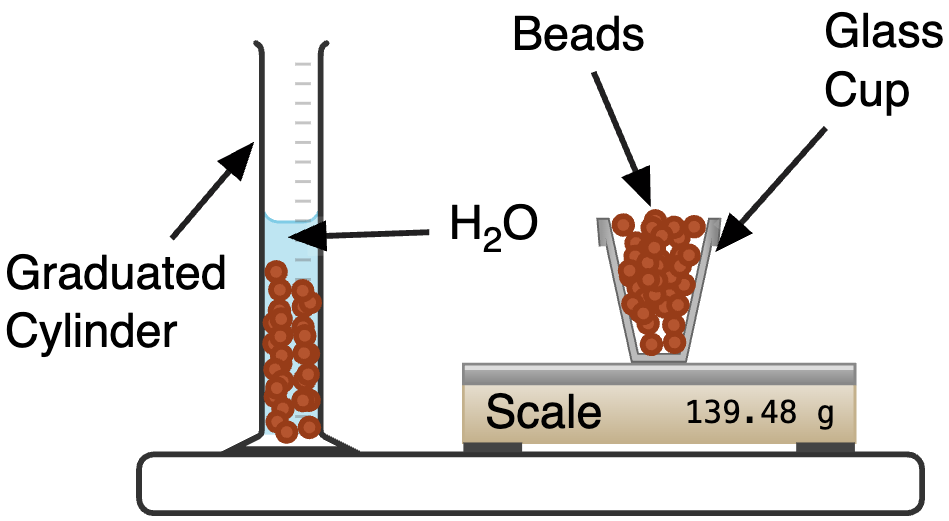
\includegraphics[width=4in]{images/setup.png}
     \caption{A diagram of our experimental setup}
     \label{fig:setup}
 \end{figure}


\section{Procedure}

We were instructed to estimate the number of beads in the jar by two different methods, so we started with the most readily apparent. We dumped the beads into the graduated cylinder to store them, and then measured the mass of the empty glass jar. We then put the beads back into the glass jar and measured the weight of the entire system. Then we placed the small plastic jar cap on the scale to secure beads, tared the scale, and measured the weight of 10 sample beads, averaging it. We then used this average to estimate the number of beads in the jar.

The second method of estimation we used was to measure the volume and displacement of the beads in water, the idea of Archimedes fame. We began by filling the cylinder with $\approx$ 60 mL of water (an arbitrary yet round amount), added the beads, and measured the level of the water, subtracting to get the volume of the beads. After using the set of calipers to measure then average the diameter of 10 beads, we used the average bead volume to calulate the number of beads in the water. 

We repeated both of these processes multiple times to ensure consistency and accuracy.

 \begin{figure}[h]
     \centering
     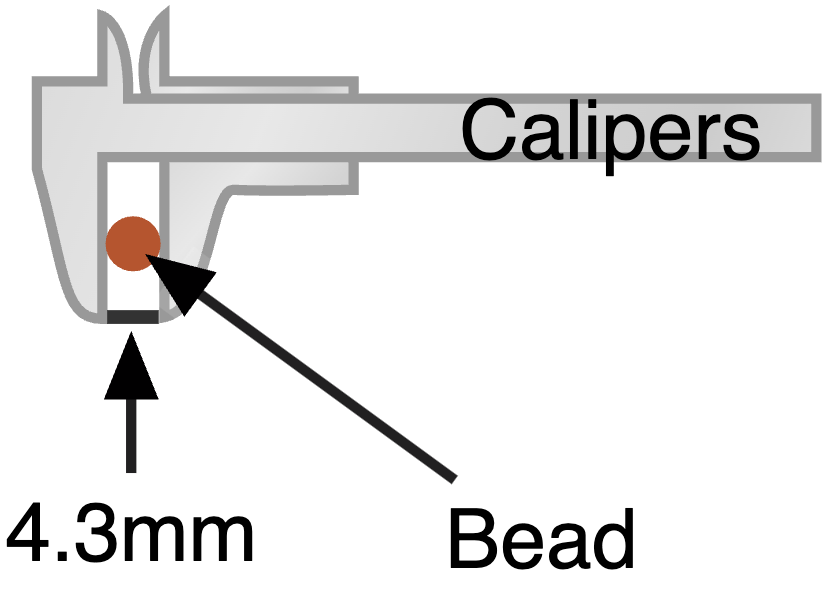
\includegraphics[width=4in]{images/measure.png}
     \caption{A diagram of using calipers to measure diameter}
     \label{fig:setup}
 \end{figure}

\section{Results}

For our first method, we measured the mass of the empty glass jar to be 9.25 g, and the mass of the glass jar full of beads to be 139.48 g. From this, we concluded that the mass of the beads was $\mathbf{130.23}\textbf{ g}$. To make this data useful, we measured the mass of 10 sample beads and averaged them to get the average mass of a bead.
\begin{equation*}
    m_\text{AVG}=\frac{\sum_{i=1}^{10} m_i}{10} = \frac{0.35+0.34+0.34+0.34+0.34+0.33+0.34+0.34+0.34+0.34}{10}=\mathbf{0.34} \textbf{ g}
\end{equation*}

We then divided the mass of all the beads by the average bead mass.
\begin{equation*}
    \frac{130.23 \text{ g}}{0.34 \text{ g}}\approx \mathbf{383 \textbf{ beads}}
\end{equation*}

For our second method, we measured the original amount of water in the graduated cylinder to be 59.3 mL, measured from the bottom of the meniscus. We then carefully poured the beads into the cylinder, then measured the volume of water to be 76.5 mL, yielding a bead volume of $\mathbf{17.2} \textbf{ mL}$. To find the volume of the average bead, we began by using calipers to measure the diameters of 10 beads.

\begin{equation*}
    d_\text{AVG}=\frac{\sum_{i=1}^{10} d_i}{10} = \frac{4.3+4.3+4.4+4.3+4.3+4.2+4.3+4.3+4.3+4.3}{10}=\mathbf{4.3} \textbf{ mm}
\end{equation*}

We used the equation for the volume of a sphere to estimate the average volume of a bead.

\begin{equation*}
    V=\frac{4}{3}\pi r^3 = \frac{4}{3}\pi \left(\frac{4.3}{2}\right)^3 = 42 \text{ mm}^3 = 0.042 \text{ cm}^3 = \mathbf{0.042}\textbf{ mL}
\end{equation*}

Now we just divide the volume of all the beads by the average for one bead.

\begin{equation*}
    \frac{17.2 \text{ g}}{0.043 \text{ g}}\approx \mathbf{410 \textbf{ beads}}
\end{equation*}

However, since this result seemed significantly different, we attempted to get a more accurate measurement of each bead's volume by measuring the water displaced by our 21 sample beads. We repeated the same procedure as before, and measured 21 beads to displace 0.9 mL of water, yielding $\mathbf{0.043} \frac{\textbf{mL}}{\textbf{bead}}$, which was the same measurement as via diameter, telling us this was an accurate number.

\begin{table}[h]
\centering
\begin{tabular}{lll}
                                        & Mass                         & Volume                         \\ \cline{2-3} 
\multicolumn{1}{l|}{Jar}                & \multicolumn{1}{l|}{9.25 g}  & \multicolumn{1}{l|}{33.1 mL}   \\ \cline{2-3} 
\multicolumn{1}{l|}{Graduated Cylinder} & \multicolumn{1}{l|}{—}       & \multicolumn{1}{l|}{100 mL}    \\ \cline{2-3} 
\multicolumn{1}{l|}{Beads}              & \multicolumn{1}{l|}{130.23 g} & \multicolumn{1}{l|}{17.2 mL}   \\ \cline{2-3} 
\multicolumn{1}{l|}{Single Bead}        & \multicolumn{1}{l|}{0.34 g}  & \multicolumn{1}{l|}{0.042 mL} \\ \cline{2-3} 
\end{tabular}
\caption{A table of our mass and volume measurements}
\label{tab:measure}
\end{table}

\pagebreak
\section{Conclusions}

While our measurement was not too imprecise, with only a 6.8\% difference.($\frac{|383-410|}{\frac{383+410}{2}}\times100 = 6.82$), there remains some source of error. Likely contributors would be the fact that trace amount of metal dust were present in the original jar of beads, and these we not incorporated into our average weight calculation. Also, when we submerged the beads in water, their rough surfaces likely held small amount of water, changing the weight and volume slightly. Theoretically the volume measurement should have been more accurate, due to largely ignoring any tiny particulates, however, our measuring accuracy in the graduated cylinder was less accurate than the electronic scale due to the presence of a meniscus and the lack of fine-grained tick marks. The volume measurement is also more volatile as a change by even $\frac{1}{1000}$ of a cubic centimeter changes the answer by dozens of beads, while the weight measurement is easier to average. While both methods provide valuable insight, neither was perfectly executed and could be improved by better measuring devices.


% \bibliographystyle{unsrtnat}
% \bibliography{references}

\end{document}
